\documentclass[11pt, a4paper]{article}
\usepackage[utf8]{inputenc}
\usepackage{fullpage}
\usepackage{graphicx}
\usepackage{markdown}
\usepackage[hidelinks]{hyperref,xcolor}
\renewcommand\UrlFont{\color{blue}\rmfamily}

\usepackage[backend=biber]{biblatex}
\addbibresource{library.bib}
\title{Project Plan\\Remote Water Sensing using UAVs}
\author{Robin \textsc{Westerik}}

\newcommand{\supervisors}{Jan \textsc{Bollen}\\Harry \textsc{Futselaar}}
\newcommand{\timePeriod}{February 2022 - June 2022}
\newcommand{\resourcesPlanned}{800 hours (40h per week)}
\newcommand{\homepage}{\url{https://github.com/organizations/remotewatersensing/}}
\date{\today}

\makeatletter{}

\begin{document}

\begin{titlepage}
  	\newcommand{\HRule}{\rule{\linewidth}{0.3mm}}
	\center
	\textsc{\LARGE Saxion University of Applied Sciences}\\[1.5cm]
	\textsc{\Large International Water Technology}\\[0.5cm]
	\textsc{\large Applied Computer Science Graduation Project}\\[0.5cm]
	\HRule\\[0.4cm]
	{\huge\bfseries \@title}\\[0.4cm]
	\HRule\\[1.5cm]

	%Author(s)
	\begin{minipage}{0.4\textwidth}
		\begin{flushleft}
			\large
			\textit{Author(s)}\\
			\@author % Your name
		\end{flushleft}
	\end{minipage}
	~
	\begin{minipage}{0.4\textwidth}
		\begin{flushright}
			%\large
			%\textit{Supervisor(s)}\\
			%\supervisors
		\end{flushright}
	\end{minipage}
	
% 	If you don't want a supervisor, uncomment the two lines below and comment the code above
% 	{\large\textit{Author(s)}}\\
% 	\@author % Your name

	%Date
	\vfill\vfill
		{\large\today}
    \vfill\vfill
    
    \footnotesize{Time period: \timePeriod}
    \\[0.3cm]
    \footnotesize{Resources planned: \resourcesPlanned}
    \vfill
    \homepage
    
    \vfill
    
    \begin{tabular}{ | l | l | l | l |}
    \hline
    \textbf{Version} & \textbf{Date of change} & \textbf{What is changed?} & \textbf{The reason for the change} \\ \hline
    0.1 & 03-02-2022 & templating & \\
    0.2 & 03-02-2022 & added project result & \\
    0.21 & 07-02-2022 & edited project result & added research question\\
    0.3 & 07-02-2022 & added project activities &\\
    0.4 & 07-02-2022 & added project boundaries &\\
    0.5 & 08-02-2022 & added interim results, quality &\\
    \hline
\end{tabular}
	
	\vfill\vfill
	
\includegraphics[width=0.4\textwidth]{./saxionlogo.png}
	\vfill
	 
	\vfill
	
\end{titlepage}


\tableofcontents
\pagebreak

\section{Background}
This project proposal has been brought forward by an idea of the International Water Technology lectorate at the Saxion University of Applied Sciences. The project will be carried out in collaboration with PERNAM JSC, a specialist in water treatment solutions in Vietnam. They are specialized in the design, engineering, and construction of water treatment technologies for groundwater, surface, and brackish water. Ton Duc Thang University, a public research university located in Ho Chi Minh City, will further accommodate the project when possible by providing expert advice and practical necessities. 

As this project will be a first of potential following projects, emphasis is laid on developing an open source and well documented foundation so that future parties can build on this project in the future. Completing this project could be a start of providing smarter water sensing solutions which in turn could benefit current water filtration solutions of Pernam as well as help with the water availability issues around Ho Chi Minh City.

\section{Project Result}
Monitoring surface level water is vital for providing feedback to water filtration solutions. Having more autonomous ways to monitor the water quality will lead to less man hours spent manually measuring the water.

The objective during this graduation project is to explore new ways in which water can be autonomously monitored by using unmanned aerial vehicles (drones). While it is impossible to know in advance exactly what the end product would entail, it would allow users to measure various water quality variables across an area by using unmanned aerial vehicles and various different water quality sensor concepts.

Future projects could mature by for example improving a specific sensor concept or by using past data to automatically determine the best filtration settings.

\section{Project Activities}

\section{Project Boundaries}

\section{Interim Results}

\section{Quality}

\section{Project Organization}

\section{Planning and Scheduling}

\section{Costs and Benefits}

\section{Risks}

\begin{figure}[h]
    \center
    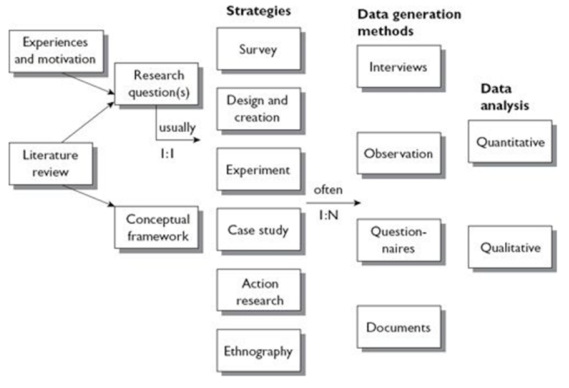
\includegraphics[width=0.5\textwidth]{research-strategies.png}
    \caption{Research strategies \cite{oates2005researching}}
    \label{fig:research_strategies}
\end{figure}

% References
\printbibliography 
\pagebreak
%Remove excerpt when publishing

\markdownInput{roelgrit.md}
\end{document}
